\documentclass{beamer}

\usepackage{tikz}
\usepackage{graphicx}
\usepackage[table, x11names]{xcolor}
\usepackage{xstring}
\usepackage{etoolbox}
\usepackage{tabularx}
\usepackage[export]{adjustbox}

\newcommand{\Date}{}

\newcommand{\setDate}[1]{\renewcommand{\Date}{#1}}

\useinnertheme{default}
\useoutertheme{default}
\usecolortheme{default}

\definecolor{aziendaPrimary}{RGB}{84, 150, 104}
\setbeamercolor{structure}{fg=aziendaPrimary}
\setbeamercolor{frametitle}{bg=aziendaPrimary!10,fg=aziendaPrimary}

% rimuovere i simboli di navigazione
\setbeamertemplate{navigation symbols}{}

% pagina iniziale
\setbeamertemplate{title page}{
  \vspace{2em}
  \begin{center}
    \begin{minipage}{0.3\textwidth}
      \centering
      
\includegraphics[height=2.1cm, left]{./logounipd.png}
    \end{minipage}
    \begin{minipage}{0.3\textwidth}
      \centering
      
\includegraphics[height=2.5cm, center]{../logo-crop.pdf}
    \end{minipage}
    \begin{minipage}{0.3\textwidth}
      \centering
      
\includegraphics[height=2cm, right]{./logoview4life.png}
    \end{minipage}
  \end{center}
  \begin{center}
      {\usebeamerfont{title}\color{black}\textbf{\inserttitle}\par}
    \vspace{0.5em}
    {\usebeamerfont{date}\insertauthor\par}
    {\usebeamerfont{date}\Date\par}
  \end{center}
}

% footer
\setbeamertemplate{footline}{
  \vspace{2ex}
  \hbox{
    \begin{minipage}[t]{0.40\paperwidth}
      \hspace*{0.5em}
      \raggedright\usebeamerfont{footline}{Progetto View4Life}
    \end{minipage}%
    \begin{minipage}[t]{0.20\paperwidth}
      \centering\usebeamerfont{footline}Slide \insertframenumber{} di \inserttotalframenumber
    \end{minipage}%
    \begin{minipage}[t]{0.40\paperwidth}
      \hfill
      \insertshortauthor
      \hspace*{0.8em}
      \raisebox{-0.25\height}{
\includegraphics[width=0.7cm]{../logo-crop.pdf}}
      \hspace*{1.3em}
    \end{minipage}
  }
  \vspace{0.8ex}
}

\usepackage[absolute,overlay]{textpos}
\definecolor{flagColor}{RGB}{0, 191, 99}
\definecolor{bgColor}{RGB}{27,77, 52}

\title{Progetto View4Life del corso \\ di Ingegneria del Software}
\author{Presentazione del \textit{MVP}}
\setDate{09/04/2026}

\begin{document}

{
\setbeamertemplate{footline}{}
\begin{frame}                                
  \titlepage
\end{frame}
}

\begin{frame}{L'obiettivo del progetto}
  % \begin{textblock*}{2cm}(10.5cm,0.5cm)
  %   \includegraphics[width=2cm]{immagine}
  % \end{textblock*}
  Sviluppare un applicativo \textit{web} per permettere la gestione delle residenze protette da parte del personale sanitario
  e dell'amministratore, tramite l'uso dei dispositivi \textit{IoT} della gamma \textit{View Wireless}. \\
  In particolare, l'applicativo deve:
  \begin{itemize}                                
    \item Visualizzare le informazioni dei vari \textbf{dispositivi};
    \item gestire gli stati degli \textbf{allarmi}, che verranno presi in carico dal personale sanitario;
    \item visualizzare le \textbf{\textit{analytics}} relative alla piattaforma e agli impianti, con relativi suggerimenti
          per il \textbf{risparmio energetico};
    \item visualizzare una \textbf{\textit{dashboard}} contenente le informazioni principali (stato dispositivi, allarmi attivi, ...).
  \end{itemize}
\end{frame}


\begin{frame}{Avanzamento fino ad oggi}
  \centering
  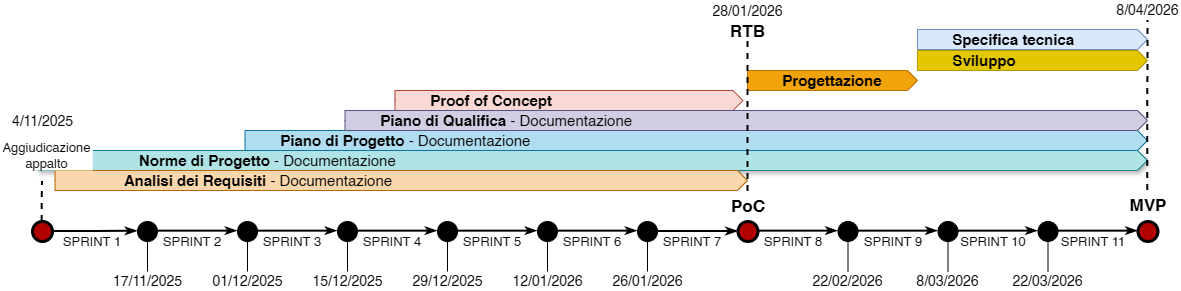
\includegraphics[                                
    width=\textwidth,
    height=\textheight,
    keepaspectratio
  ]{stato_avanzamento.drawio.png}
\end{frame}

\begin{frame}{Autenticazione(1/2): funzionalità }
  Il sistema prevede l'utilizzo da parte di due categorie di utenti:
  \begin{itemize}                                
    \item Amministratore,
    \item Operatore Socio Sanitario.
  \end{itemize}
  L'Amministratore ha accesso ad alcune funzionalità riservate ed è responsabile del collegamento
  all'account \textit{myVimar}, che permette la corretta interazione con i dispositivi associati.
  
\end{frame}

\begin{frame}{Autenticazione(2/2): interfaccia}
  \centering
  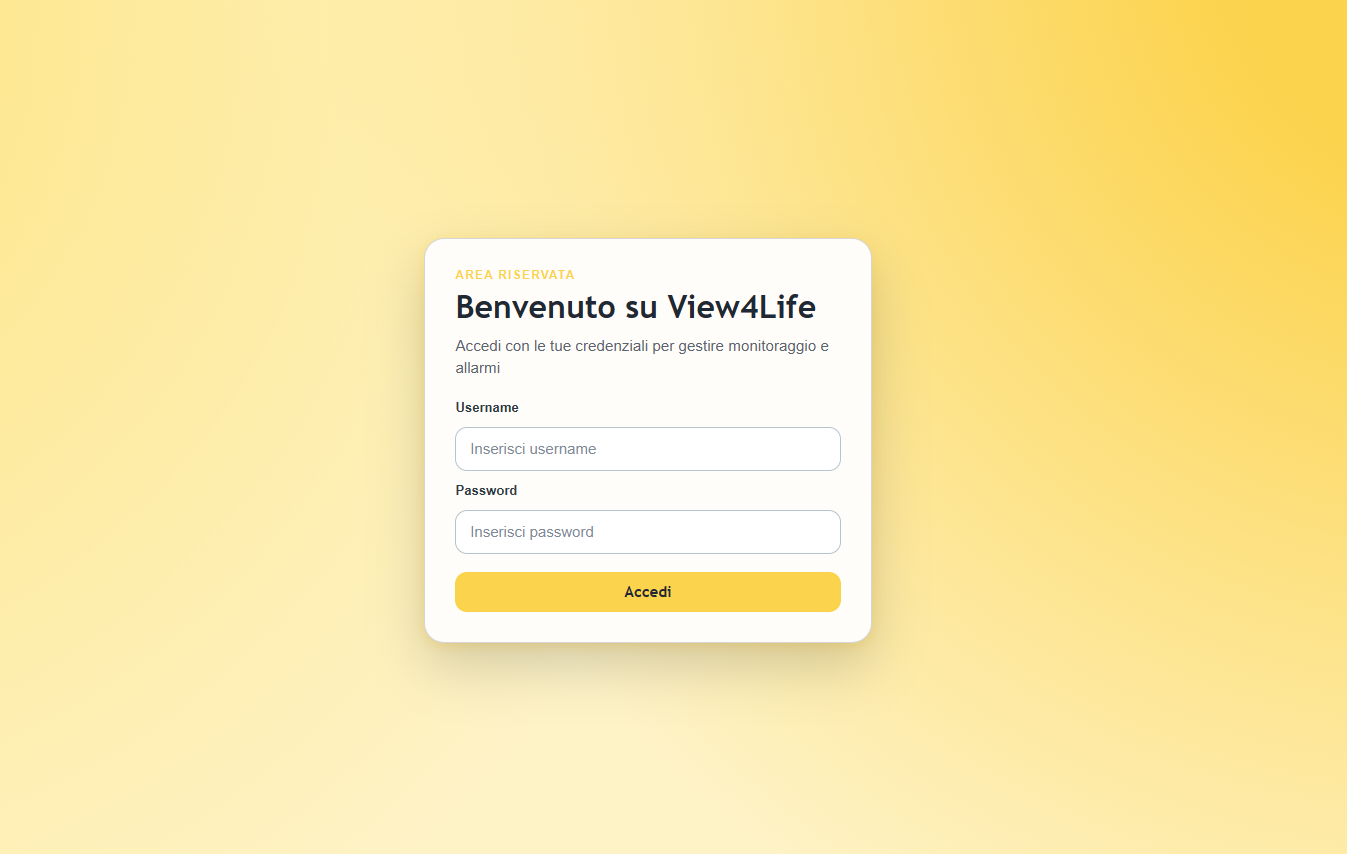
\includegraphics[                                
    width=\textwidth,
    height=\textheight,
    keepaspectratio
  ]{login.png}
\end{frame}

\begin{frame}{Dashboard(1/2): funzionalità }
  La dashboard è la schermata principale dell'applicativo e permette di ottenere una panoramica dello stato
  dell'impianto.\\
  Prevede la possibilità di:
  \begin{itemize}                                
    \item Visualizzare la lista limitata degli allarmi attivi con priorità maggiore;
    \item Prendere in carico un allarme;
    \item consultare i consumi energetici e le statistiche sugli allarmi;
    \item visualizzare una panoramica strutturale dell'appartamento e i dispositivi contenuti.
  \end{itemize}
\end{frame}

\begin{frame}{Dashboard(2/2): interfaccia}
  \centering
  
\includegraphics[                                
    width=\textwidth,
    height=\textheight,
    keepaspectratio
  ]{dashboard.png}
\end{frame}

\begin{frame}{Gestione Allarmi(1/2): funzionalità }
  La sezione di gestione allarmi allarmi è rivolta agli Operatori Socio Sanitari e permette di:
  \begin{itemize}                                
    \item Visualizzare la lista completa degli allarmi attivi.
    \item Prendere in carico un allarme.
  \end{itemize}
\end{frame}

\begin{frame}{Gestione Allarmi(2/2): interfaccia }
  \centering
  
\includegraphics[                                
    width=\textwidth,
    height=\textheight,
    keepaspectratio
  ]{gestione-allarmi.png}
\end{frame}

\begin{frame}{Configurazione Allarmi (1/3): funzionalità}
  La sezione Configurazione allarmi è riservata all'amministratore e ha lo scopo di fornire gli strumenti 
  per definire il comportamento degli allarmi all'interno dell'impianto.\\
  Prevede la possibilità di:
  \begin{itemize}                                
    \item Visualizzare la lista delle regole degli allarmi;
    \item Eliminare, disabilitare le regole o modificarne le caratteristiche (ad esempio priorità, soglia, orario d'attivazione, ...).
    \item Creare nuove regole tramite modulo dedicato.
  \end{itemize}
\end{frame}

\begin{frame}{Configurazione Allarmi(2/3): interfaccia }
  \centering
  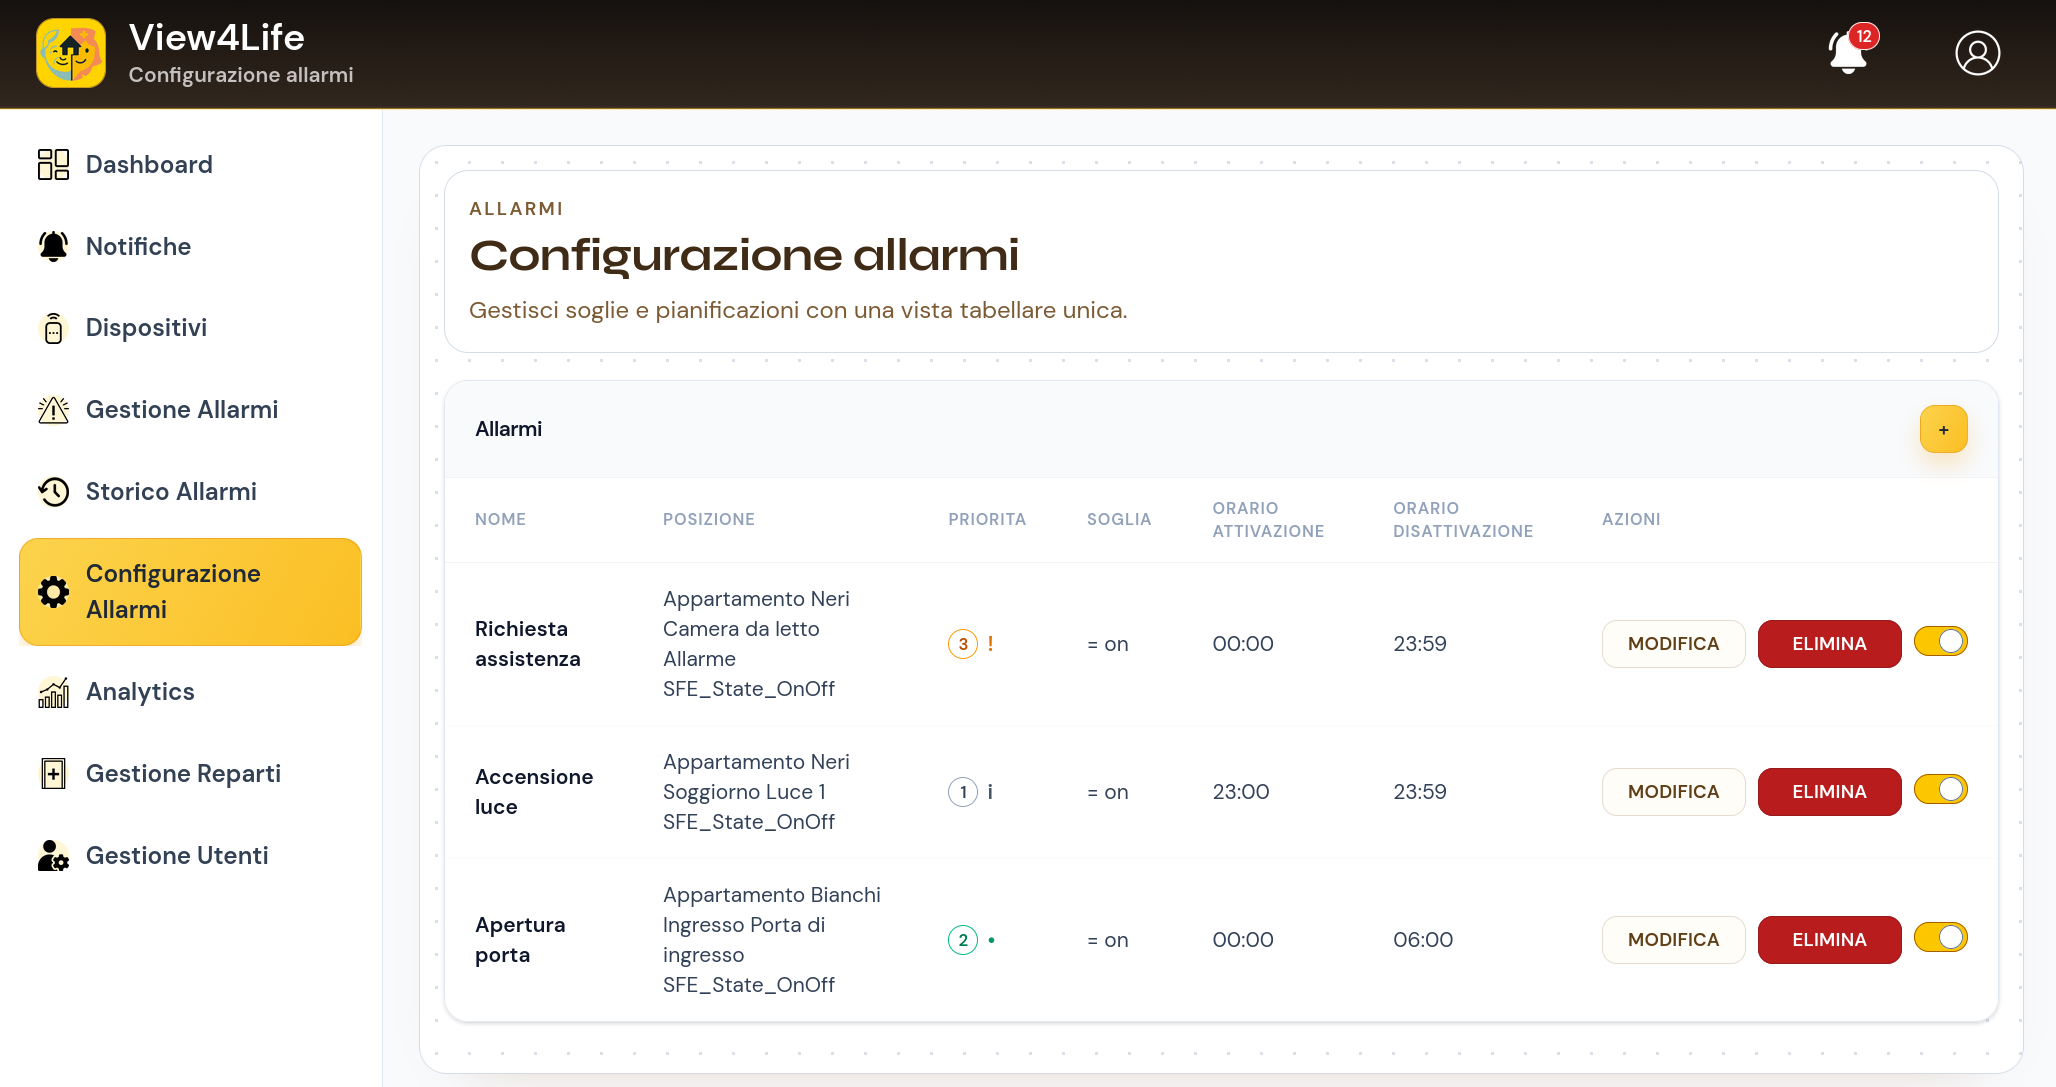
\includegraphics[                                
    width=\textwidth,
    height=\textheight,
    keepaspectratio
  ]{configurazione-allarmi.png}
\end{frame}

\begin{frame}{Configurazione Allarmi(3/3): interfaccia }
  \centering
  
\includegraphics[                                
    width=0.9\textwidth,
    height=0.9\textheight,
    keepaspectratio
  ]{configurazione-allarme-1.png}
\end{frame}

\begin{frame}{Analytics(1/2): funzionalità }
  Le Analytics consistono in un cruscotto informativo contenente statistiche sui dati ottenuti dai dispositivi degli impianti. \\
  Sulla base di questi vengono generati dei suggerimenti tramite LLM.
  \begin{itemize}                                
    \item Visualizzare i grafici relativi alle statistiche di un impianto.
    \item Visualizzare i suggerimenti per il risparmio energetico.
          
  \end{itemize}
\end{frame}

\begin{frame}{Analytics(2/2): interfaccia }
  \centering
  
\includegraphics[                                
    width=\textwidth,
    height=\textheight,
    keepaspectratio
  ]{analytics.png}
\end{frame}

\begin{frame}{Altre funzionalità dell'Amministratore}
  La figura dell'amministratore ha inoltre accesso alle seguenti funzionalità:
  \begin{itemize}                                
    \item Gestione Reparti: permette di amministrare le relazioni reparto-appartamento e reparto-operatori;
    \item Gestione Utenti: permette la creazione e l'eliminazione di utenti.
  \end{itemize}
\end{frame}

\begin{frame}{Modello architetturale}
  \centering
  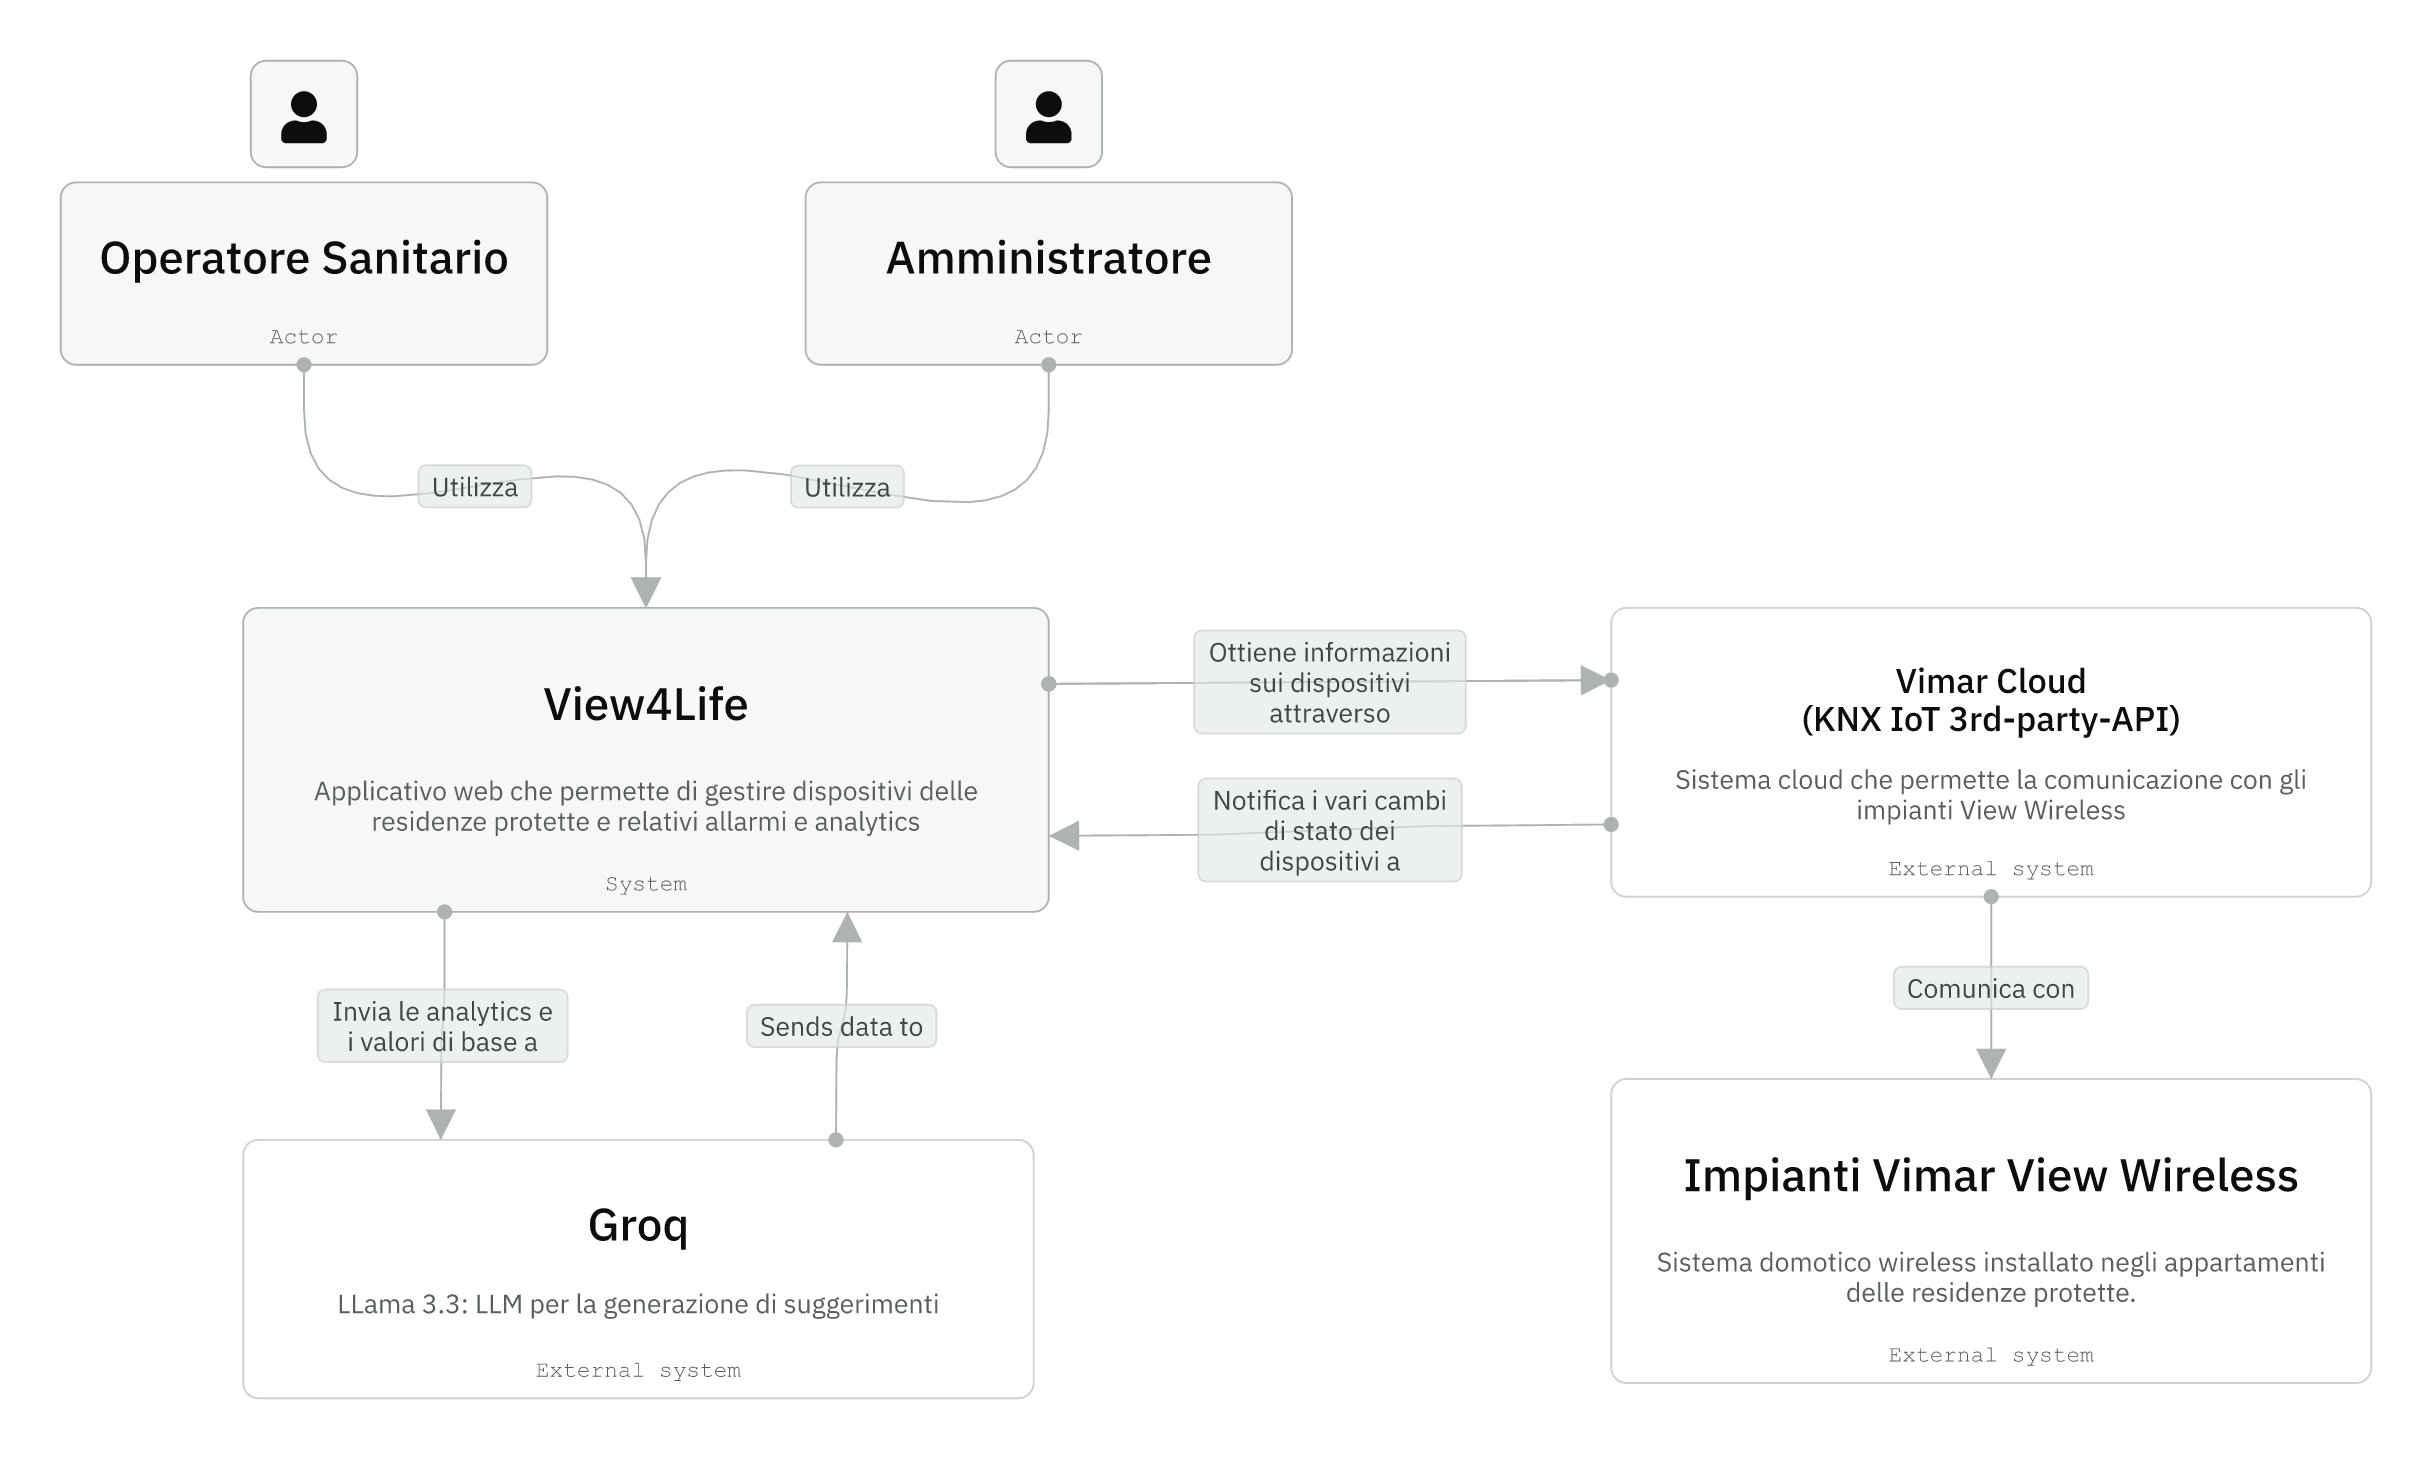
\includegraphics[                                
    width=\textwidth,
    height=0.8\textheight,
    keepaspectratio
  ]{c4-lv1.png}
\end{frame}

\begin{frame}{Aspetti positivi del progetto}
  Il gruppo, in riferimento al progetto, ha individuato i seguenti aspetti positivi:
  \begin{itemize}                                
    \item Sviluppo delle competenze di comunicazione e collaborazione 
          all'interno di un team strutturato.
    \item Acquisizione di nuove conoscenze tecniche legate 
          alle tecnologie adottate.
    \item Realizzazione di un prodotto con impatto concreto, 
          grazie alla collaborazione con un'azienda reale.
    \item Sperimentazione della metodologia Scrum per la gestione del progetto, 
          con organizzazione del lavoro in sprint.
    \item Esposizione a un flusso di lavoro professionale, 
          che include versionamento, documentazione e coordinamento del team.
  \end{itemize}
\end{frame}

\begin{frame}{Aspetti negativi del progetto}
  Gli aspetti negativi riscontrati dal gruppo durante il progetto sono:
  \begin{itemize}                                
    \item Leggero disallineamento sui requisiti di progetto tra team e Proponente.
    \item Difficoltà nella definizione di previsioni corrette.
    \item Difficoltà nel rispetto delle scadenze.
    \item Sporadica mancanza di comunicazione interna, che ha comunque provocato rallentamenti.
  \end{itemize}
\end{frame}

\end{document}